\RequirePackage{currfile} 

\documentclass[aspectratio=169]{beamer}

%%%%%%%%%%%%%%%%%%%%%%%%%%%%%%%%%%%%%%%%%
% Beamer Presentation
% LaTeX Template
% Version 1.0 (10/11/12)
%
% This template has been downloaded from:
% http://www.LaTeXTemplates.com
%
% License:
% CC BY-NC-SA 3.0 (http://creativecommons.org/licenses/by-nc-sa/3.0/)
%
%%%%%%%%%%%%%%%%%%%%%%%%%%%%%%%%%%%%%%%%%

%----------------------------------------------------------------------------------------
%	PACKAGES AND THEMES
%----------------------------------------------------------------------------------------




\mode<presentation> {

% The Beamer class comes with a number of default slide themes
% which change the colors and layouts of slides. Below this is a list
% of all the themes, uncomment each in turn to see what they look like.

%\usetheme{default}
%\usetheme{AnnArbor}
% \usetheme{Antibes}
% \usetheme{Bergen}
%\usetheme{Berkeley}
\usetheme{Berlin}
%\usetheme{Boadilla}
% \usetheme{CambridgeUS}
%\usetheme{Copenhagen}
%\usetheme{Darmstadt}
%\usetheme{Dresden}
%\usetheme{Frankfurt}
%\usetheme{Goettingen}
%\usetheme{Hannover}
%\usetheme{Ilmenau}
%\usetheme{JuanLesPins}
%\usetheme{Luebeck}
%\usetheme{Madrid}		
%\usetheme{Malmoe}
%\usetheme{Marburg}
%\usetheme{Montpellier}
%\usetheme{PaloAlto}
%\usetheme{Pittsburgh}
%\usetheme{Rochester}
%\usetheme{Singapore}
%\usetheme{Szeged}
% \usetheme{Warsaw}

% As well as themes, the Beamer class has a number of color themes
% for any slide theme. Uncomment each of these in turn to see how it
% changes the colors of your current slide theme.

% \usecolortheme{albatross}
% \usecolortheme{beaver}
% \usecolortheme{beetle}
% \usecolortheme{crane}
% \usecolortheme{dolphin}
% \usecolortheme{dove}
% \usecolortheme{fly}
\usecolortheme{lily}
% \usecolortheme{orchid}
% \usecolortheme{rose}
% \usecolortheme{seagull}
% \usecolortheme{seahorse}
% \usecolortheme{whale}
% \usecolortheme{wolverine}

%\setbeamertemplate{footline} % To remove the footer line in all slides uncomment this line
%\setbeamertemplate{footline}[frame number] % To replace the footer line in all slides with a simple slide count uncomment this line

%\setbeamertemplate{navigation symbols}{} % To remove the navigation symbols from the bottom of all slides uncomment this line

% \setbeamercovered{transparent} % Fait apparaître les animations en grisé (utile pour la conception, mais peut être commenté lors de la remise du document final)

% Pour utiliser une police à empattements partout
\renewcommand{\familydefault}{\sfdefault}

% Pour rajouter la numérotation des frames dans les pieds de page
\newcommand*\oldmacro{}%
\let\oldmacro\insertshorttitle%
\renewcommand*\insertshorttitle{%
  \oldmacro\hfill%
  \insertframenumber\,/\,\inserttotalframenumber}

}

\usepackage{graphicx} % Allows including images
\usepackage{booktabs} % Allows the use of \toprule, \midrule and \bottomrule in tables

\setbeamertemplate{caption}[numbered]
\newcommand\subheading[1]{%
  {\Large\bfseries#1}\par\smallskip}
\usepackage{natbib}        
\usepackage{url}           
% \usepackage[T1]{fontenc}   
% \usepackage[utf8]{inputenc}
% \usepackage[english]{babel}
\usepackage[utf8]{vietnam}
\usepackage{numprint}      

\usepackage{amsmath}       
\usepackage{mathrsfs}      
\usepackage{amssymb}       
\usepackage{amsfonts} 

\usepackage{cancel}


\usepackage{minted}
\usemintedstyle{friendly}

\usepackage{graphicx}
\usepackage{wrapfig}  

\usepackage{tikz}     

% \usepackage[framemethod=TikZ]{mdframed}
% \usepackage[T1]{fontenc}
% Ce fichier contient toutes les macros que vous pouvez avoir envie de définir 
% si vous les utilisez plusieurs fois dans le document.

\PassOptionsToPackage{svgnames}{color}

% Un environnement pour bien présenter le code informatique
\newenvironment{code}{%
\begin{mdframed}[linecolor=green,innerrightmargin=30pt,innerleftmargin=30pt,
backgroundcolor=black!5,
skipabove=10pt,skipbelow=10pt,roundcorner=5pt,
splitbottomskip=6pt,splittopskip=12pt]
}{%
\end{mdframed}
}

% Un raccourci pour composer les unités correctement (en droit)
% Exemple: $v = 10\U{m.s^{-1}}$
\newcommand{\U}[1]{~\mathrm{#1}}

% Les guillemets \ofg{par exemple}
\newcommand{\ofg}[1]{\og{}#1\fg{}}

% Le d des dérivées doit être droit: \frac{\dd x}{\dd t}
\newcommand{\dd}{\text{d}}

% La dérivée temporelle, tellement courante en physique, avec les d droits
\newcommand{\ddt}[1]{\frac{\dd #1}{\dd t}}

% Des parenthèses, crochets et accolades qui s'adaptent automatiquement à la 
% taille de ce qu'il y a dedans
\newcommand{\pa}[1]{\left(#1\right)}
\newcommand{\pac}[1]{\left[#1\right]}
\newcommand{\paa}[1]{\left\{#1\right\}}

% Un raccourci pour écrire une constante
\newcommand{\cte}{\text{C}^{\text{te}}}

% Pour faire des indices en mode texte (comme les énergie potentielles)
\newcommand{\e}[1]{_{\text{#1}}}

% Le produit vectoriel a un nom bizarre:
\newcommand{\vectoriel}{\wedge}


\title[Sinh biểu cảm khuôn mặt dựa trên phù hợp giọng nói]{\textbf{SINH BIỂU CẢM KHUÔN MẶT DỰA TRÊN PHÙ HỢP GIỌNG NÓI}}

\author{Trần Hoàng Tuấn\inst{1}, Lê Thành Sách\inst{2}}

\institute[HCMUT]{
\inst{1}%
Học viên thực hiện\\
Khoa học máy tính, đại học Bách Khoa thành phố Hồ Chí Minh
\and
\inst{2}%
Tiến sĩ hướng dẫn khoa học\\
Khoa học máy tính, đại học Bách Khoa thành phố Hồ Chí Minh }
\date{Bảo vệ đề cương luận văn, 01/2021} 

\begin{document}
\begin{frame}
\titlepage 
\end{frame}
\frame{\tableofcontents}

\section{Giới thiệu}\label{sec:intro}
\frame{\tableofcontents[currentsection]}
\begin{frame}{Giới thiệu}

\begin{itemize}
    \item Là một bài toán tạo sinh dữ liệu dạng hình ảnh dựa trên các dạng dữ liệu khác.
    \item Cho trước một vài dữ liệu về gương mặt của một người bất kỳ \textit{(hình ảnh, video ngắn)} và môt đoạn tiếng nói bất kỳ. Tạo sinh hình ảnh người đó đang nói đoạn tiếng nói đã cho một cách chân thực.
\begin{figure}[H]
    \centering
    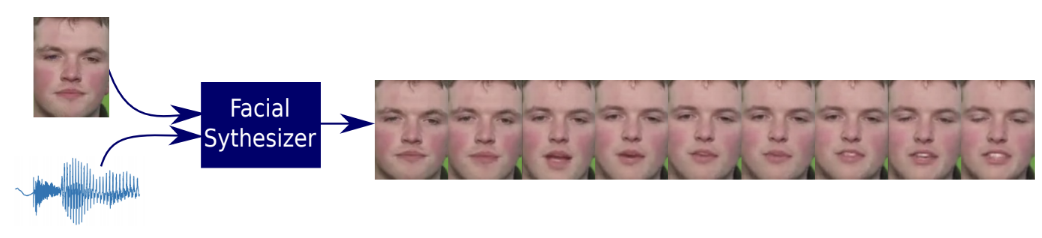
\includegraphics[width=13cm]{images/intro.png}
    \caption{Ví dụ về mô hình tạo sinh khuôn mặt}
    \label{fig:example}
\end{figure}
\end{itemize}
\end{frame}

\section{Mục tiêu, giới hạn và đối tượng của nghiên cứu}\label{sec:intro}
\frame{\tableofcontents[currentsection]}
\begin{frame}{Mục tiêu, giới hạn và đối tượng của nghiên cứu}
\begin{enumerate}
    \item <1-> \textit{Mục tiêu}: Xây dựng mô hình có thể nhận dạng các thuộc tính có độ chính xác cao.
    \item <2-> \textit{Giới hạn}: Dữ liệu là người đi bộ (đã qua bước nhận dạng), độ phân giải, kích thước của ảnh và các thuộc tính của người đi bộ.
    \item <3-> \textit{Đối tượng}: Các hướng tiếp cận, giải quyết bài toán truy tìm đối tượng, các phương pháp học máy, học sâu.
\end{enumerate}
\end{frame}


\section{Ý nghĩa thực tiễn}\label{sec:intro}
\frame{\tableofcontents[currentsection]}
\begin{frame}{Ý nghĩa thực tiễn}
\begin{itemize}
    \item Tái hiện mặt người đang nói ở nhiều thứ tiếng khác nhau
    \item Tạo sinh khuôn mặt người đại diện trong các hội nghị trực tuyến
    \item Tích hợp vào các trò chơi điện tử
    \item Giả lập trợ lý ảo có hình dáng con người
    \item Giảm bớt áp lực lên khâu hóa trang, kỹ xảo trong quá trính làm phim
\end{itemize}
\end{frame}

\section{Các công trình nghiên cứu có liên quan}\label{sec:intro}
\frame{\tableofcontents[currentsection]}

\subsection{Lip Movements Generation at a Glance\cite{chen2018}}
\begin{frame}{Lip Movements Generation at a Glance}
    \begin{figure}[H]
    \centering
    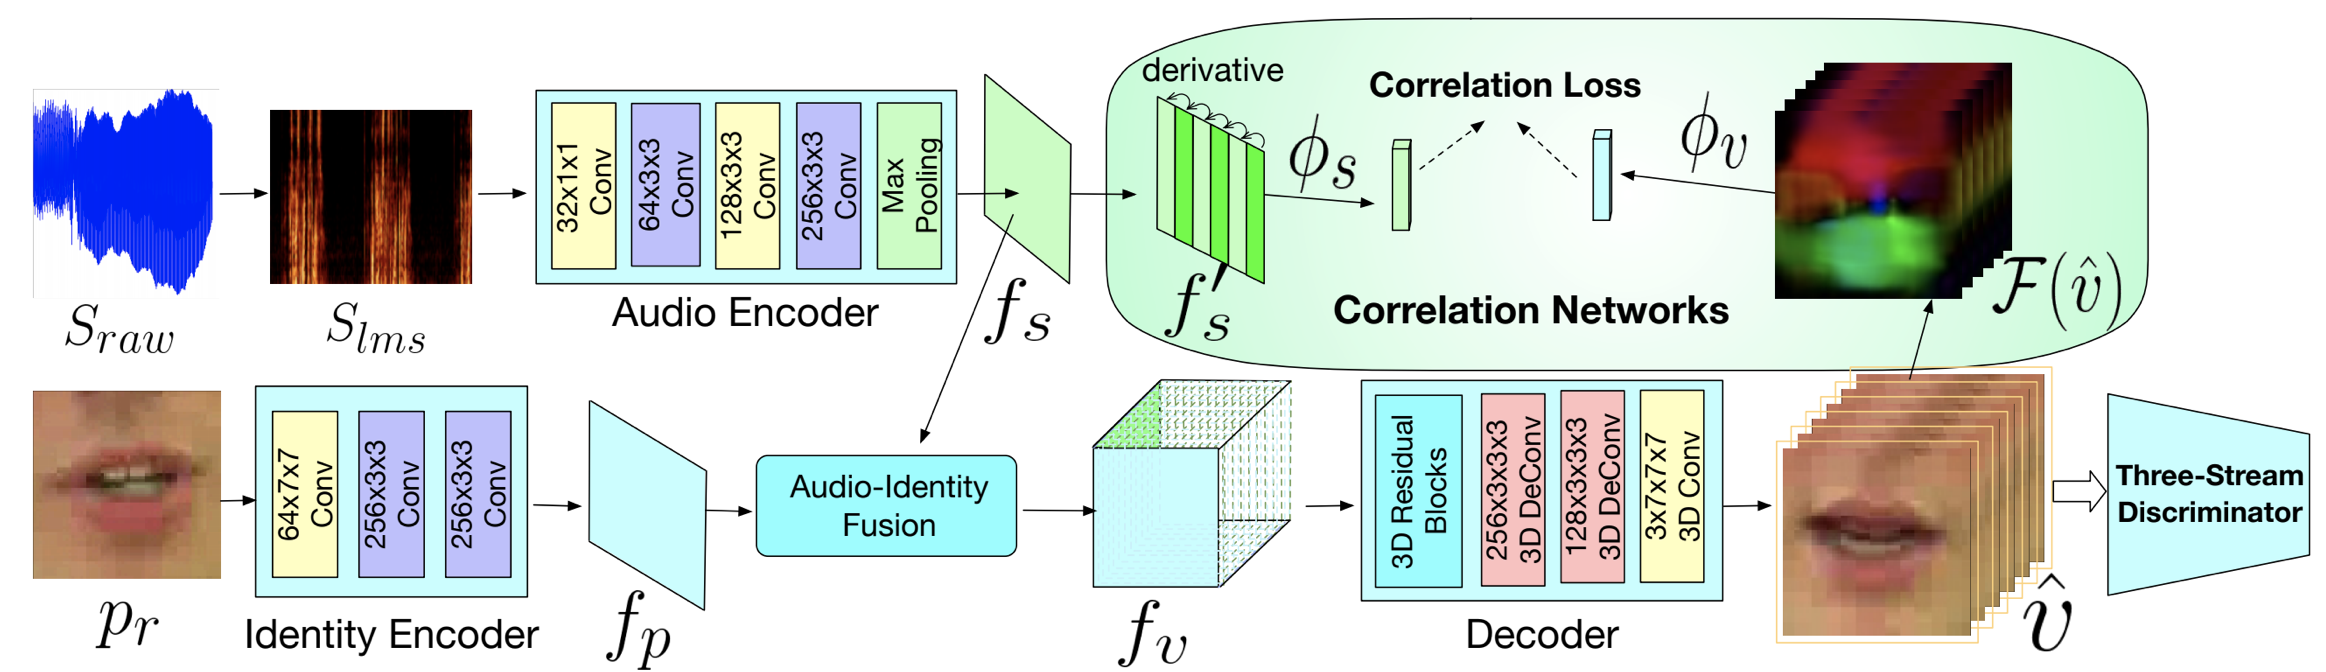
\includegraphics[width=12cm]{images/chen2018_model.png}
    \label{fig:chen2018_model}
    \caption{Kiến trúc mô hình}
    \end{figure}
\end{frame}

\begin{frame}{Lip Movements Generation at a Glance}
    \begin{figure}[H]
        \centering
        \begin{minipage}{0.48\textwidth}
            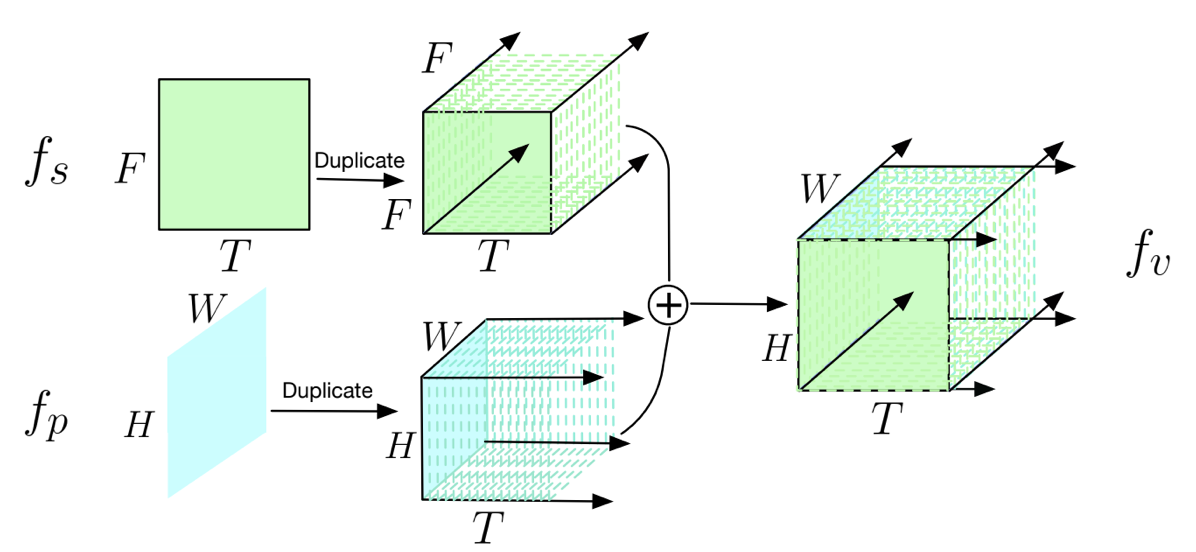
\includegraphics[width=7cm]{./images/chen2018_fusion.png}
            \caption{Phương pháp kết hợp đặc trưng hình ảnh và âm thanh}
            \label{fig:chen2018_fusion}
        \end{minipage}\hfill
        \begin{minipage}{0.48\textwidth}
            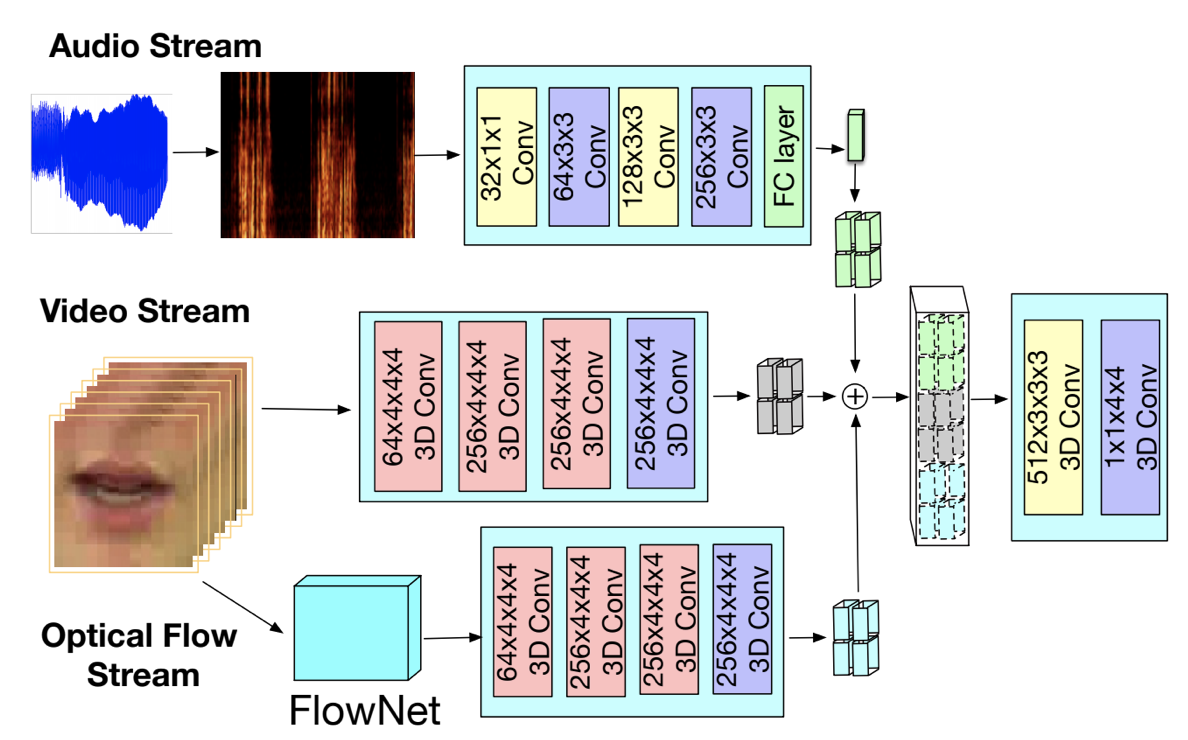
\includegraphics[width=7cm]{./images/chen2018_gans.png}
            \caption{GANs Discriminator với 3 loại đặc trưng}
            \label{fig:chen2018_gans}
        \end{minipage}
    \end{figure}
\end{frame}

\begin{frame}{Lip Movements Generation at a Glance}
    \begin{itemize}
        \item Ưu điểm
        \begin{itemize}
            \item Đưa ra các phương pháp phù hợp và tiến bộ để trích xuất và kết hợp đặc trưng hình ảnh và âm thanh
            \item Tận dụng phương pháp GANs để cải thiện chất lượng của ảnh
            được tạo sinh
        \end{itemize}
        \item Khuyết điểm
        \begin{itemize}
            \item Mạng chỉ có thể nhận vào hình ảnh tĩnh và một đoạn âm thanh có độ dài xác định (0.64s) và cho ra số khung hình tương ứng với khoảng thời gian đó (16 khung hình)
            \item Chưa chú ý đến hiện tượng nhảy hình của video được tạo sinh, mạng không có cơ chế để đảm bảo việc chuyển ảnh mượt mà, ít sai khác về độ tương phản, ánh sáng, màu sắc giữa các khung ảnh gần nhau
        \end{itemize}
    \end{itemize}
\end{frame}

\subsection{Realistic Speech-Driven Facial Animation with GANs\cite{vougioukas2020}}
\begin{frame}{Realistic Speech-Driven Facial Animation with GANs}
    \begin{figure}[H]
        \centering
        \begin{minipage}{0.48\textwidth}
            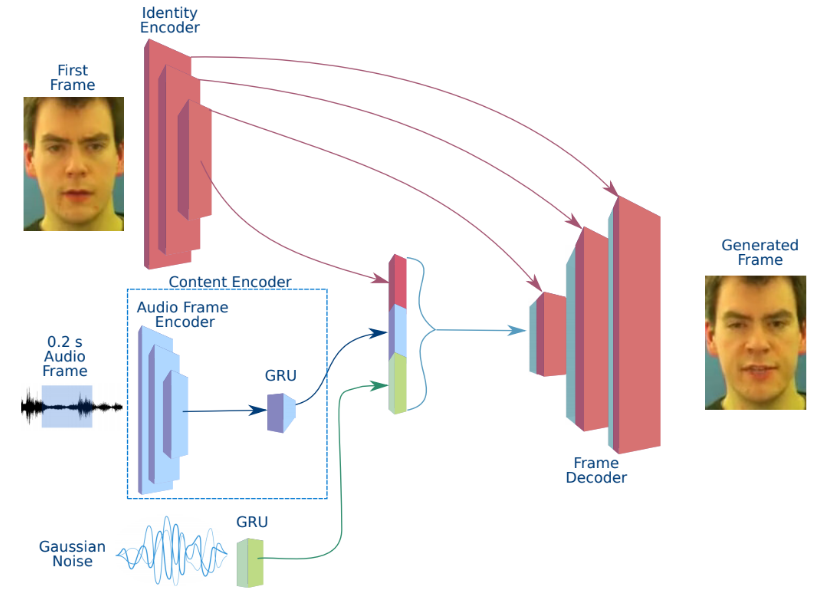
\includegraphics[width=7cm]{./images/vou2020_generator.png}
            \caption{Bộ Generator}
            \label{fig:vou2020_generator}
        \end{minipage}\hfill
        \begin{minipage}{0.48\textwidth}
            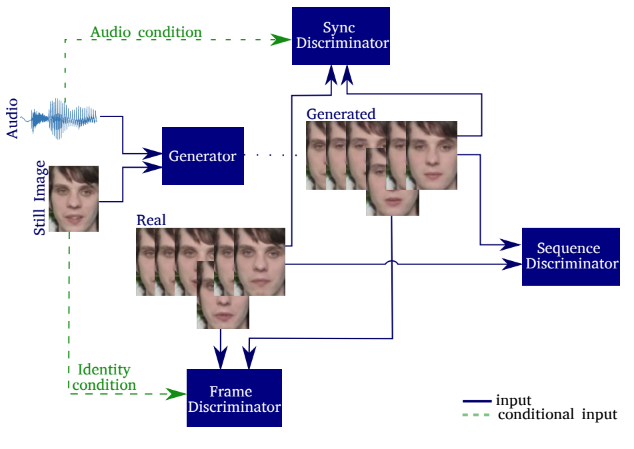
\includegraphics[width=7cm]{./images/vou2020_model.png}
            \caption{GANs Discriminator với 3 đặc trưng}
            \label{fig:vou2020_model}
        \end{minipage}
    \end{figure}
\end{frame}

\begin{frame}{Realistic Speech-Driven Facial Animation with GANs}
    \begin{figure}[H]
        \centering
        \begin{minipage}{0.48\textwidth}
            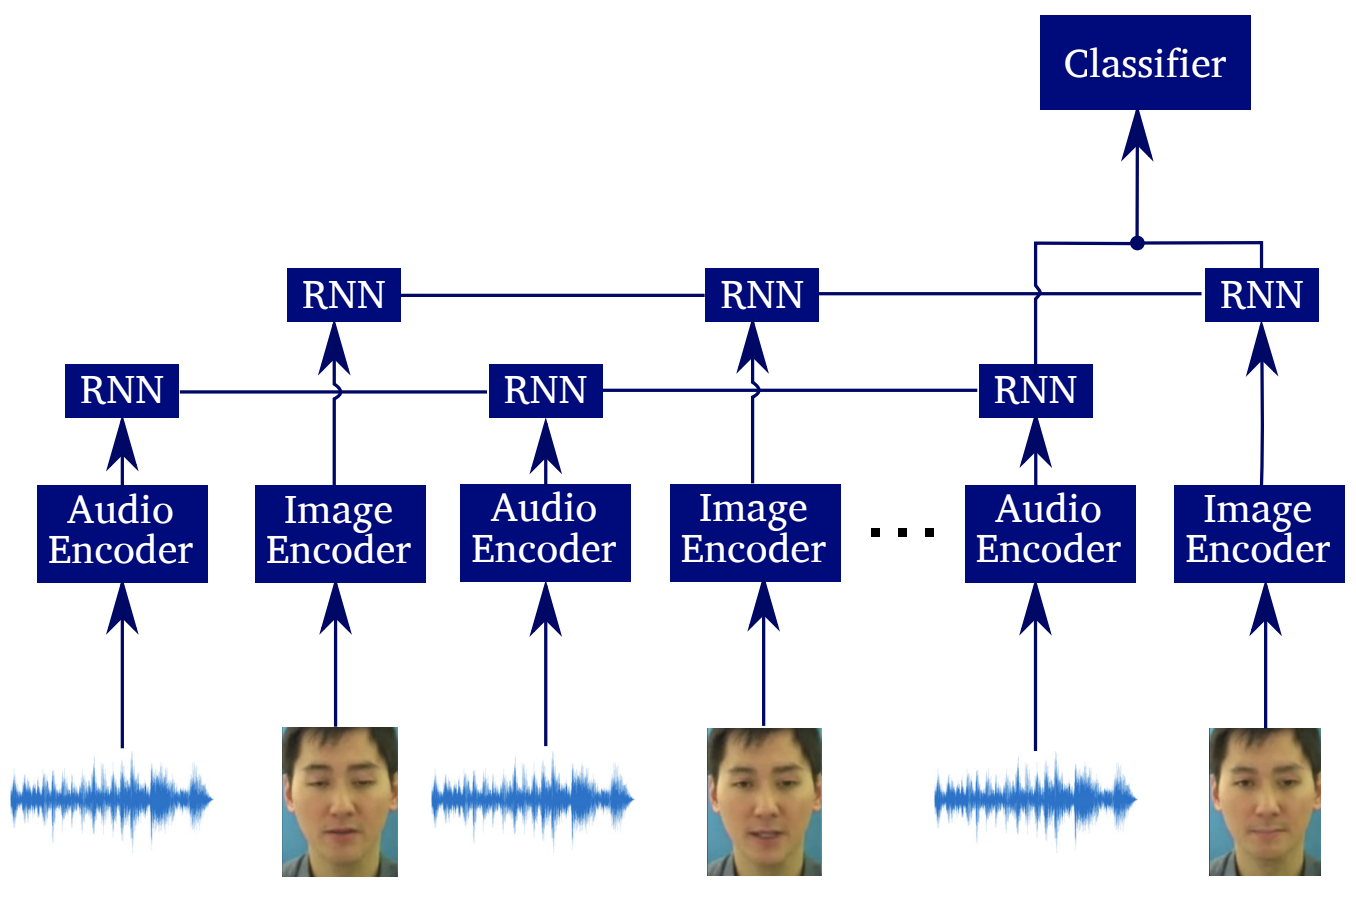
\includegraphics[width=7cm]{./images/vou2019_seq_dis.png}
            \caption{Sequence Discriminator}
            \label{fig:vou2020_generator}
        \end{minipage}\hfill
        \begin{minipage}{0.48\textwidth}
            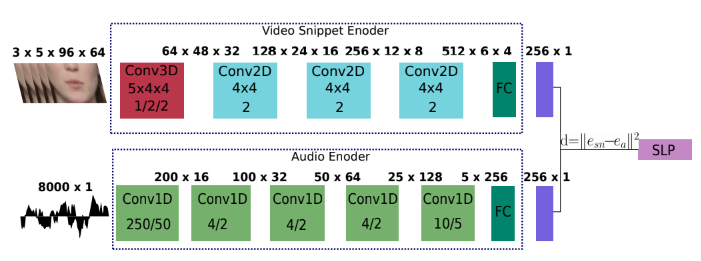
\includegraphics[width=7cm]{./images/vou2020_sync_dis.png}
            \caption{Sync Discriminator - Ba trường hợp: ảnh-âm gốc, ảnh-âm lệch, ảnh tạo sinh - âm}
            \label{fig:vou2020_model}
        \end{minipage}
    \end{figure}
\end{frame}

\begin{frame}{Realistic Speech-Driven Facial Animation with GANs}
    \begin{itemize}
        \item Ưu điểm
        \begin{itemize}
            \item Đưa ra các phương pháp tạo sinh khuôn mặt có chú ý đến khẩu hình miệng và sự mượt mà trong chuyển động giữa các khung hình
            \item Dùng xác suất ngẫu nhiên để sinh ra chuyển động ở các vị trí khác trên mặt (mắt)
            \item Hạn chế việc lệch tiếng nói nhờ Sync Discriminator
        \end{itemize}
        \item Khuyết điểm
        \begin{itemize}
            \item Chưa thể hiện được các biểu cảm trên gương mặt
            \item Chưa chú ý đến chuyển động của đầu
            \item Chưa chú trọng việc tái tạo môi trường xung quanh
            \item Không tái tạo tốt đặc điểm gương mặt của những người không nằm trong tập huấn luyện
        \end{itemize}
    \end{itemize}
\end{frame}

\section{Kế hoạch nghiên cứu}\label{sec:intro}
\frame{\tableofcontents[currentsection]}
\begin{frame}{Kế hoạch nghiên cứu}

\begin{itemize}
    \item Khảo sát, thử nghiệm một số phương pháp tạo sinh ảnh dùng cơ chế attention
    \item Khảo sát, thử nghiệm thêm một số phương pháp tạo sinh ảnh sử dụng các đặc trưng trong không gian ba chiều.
    \item Tiến hành thiết, hiện thực và kiểm chứng các kiến trúc mạng mới dựa trên những kiến thức đã thu thập được.
    \item Tổng hợp các thử nghiệm và lựa chọn kiến trúc mạng tốt nhất cho Luận văn.
    \item Viết báo cáo và bảo vệ Luận văn.
\end{itemize}
\end{frame}

\section{Kết quả dự kiến}\label{sec:intro}
\frame{\tableofcontents[currentsection]}
\begin{frame}{Kết quả dự kiến}

\begin{itemize}
    \item Xây dựng được mô hình tính toán mới, có khả năng tạo sinh hình ảnh mặt người một cách chân thật.
    \item Luận văn cũng sẽ cung cấp được các đánh giá và so sánh khách quan với các mô hình hiện tại bằng số liệu thực tế.
\end{itemize}
\end{frame}


\bibliographystyle{unsrt}
\bibliography{references}
\include{./references}



\begin{frame}
    \textbf{\LARGE{\begin{center}Thank you for your attention\end{center}}}
\end{frame}

\end{document}
